\section{Model}
\label{sec:Model}


\subsection{Q-Learning}
Q-learning learns action-reward function Q(s,a): determines how good to take an action in a particular state. In Q-learning we build memory table Q[s,a] to store Q-values for all possible combinations of s and a. We sample an action from the current state to find out reward  and new state. From the memory table, we determine the next action to take which has maximum Q(s,a).

\begin{figure}%
\centering
\includegraphics[width=0.6\columnwidth]{figures/Q-learning.png}%
\caption{Q-Learning Algorithm}%
\label{fig:datastats}%
\end{figure}


\subsection{DQN}
The number of actions we can take from current state is large and we need to observe each action space to solve this problem. We will be using Deep Q Network (DQN) to find Q(s,a). However while exploring each state space the Q value(label) will be changing each time and we will be updating model parameters to update based on new Q value each time. The newly Q value will be higher at the same time the target Q value will be move higher making it difficult for algorithm to optimize. To solve this challenges we can slow down the changing Q value using Experience replay and Target network.

We will train the neural network on subset of transitions into a buffer. From this buffer we will sample mini batch which will be stable for training. We will be buiding two neural network one to retrieve Q values while second one is to update the Q value. After a fixed intervals we will synchronize the parameters. 

\begin{figure}%
\centering
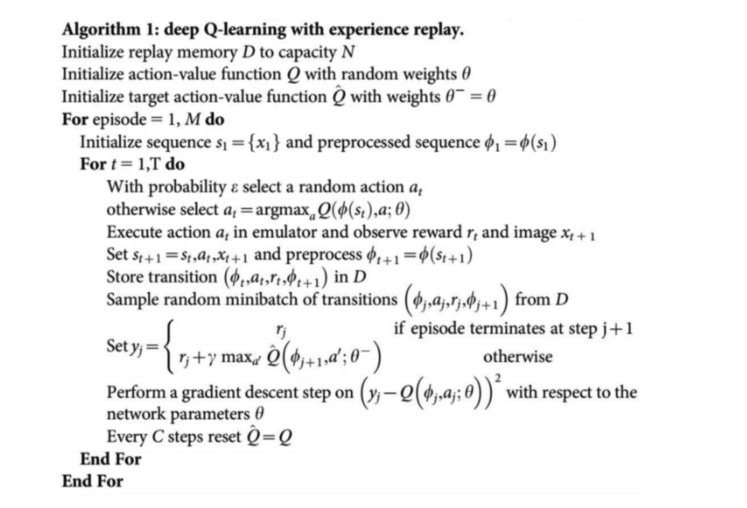
\includegraphics[width=0.6\columnwidth]{figures/DQN-ExperinceReplay.png}%
\caption{DQN with Experience Replay}%
\label{fig:datastats}%
\end{figure}


\subsection{Loss function}


DQN Uses huber loss where loss is quadratic for small values of a and linear for larger values.


\begin{figure}%
\centering
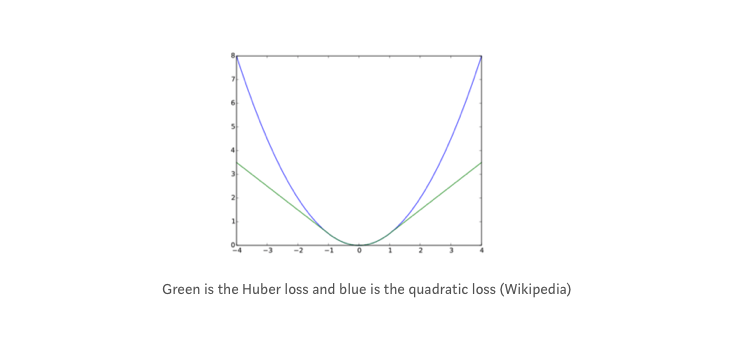
\includegraphics[width=0.6\columnwidth]{figures/loss-function.png}%
\caption{DQN loss function}%
\label{fig:datastats}%
\end{figure}


\subsection{Architecture}

Input to the DQN network is compressed video frames of 84 x 84 pixels followed by fully connected layers to compute Q value for each action.

\begin{figure}%
\centering
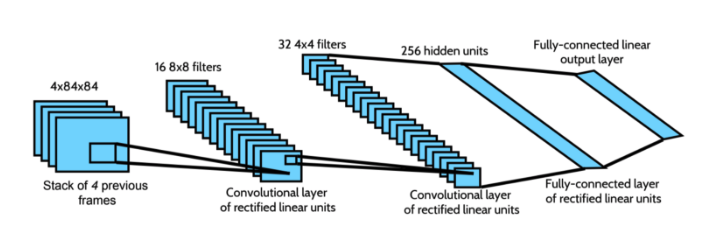
\includegraphics[width=0.6\columnwidth]{figures/DQN-architecture.png}%
\caption{DQN Architecture}%
\label{fig:datastats}%
\end{figure}




\subsection{Experiments and Evaluation}

\begin{figure}%
\centering
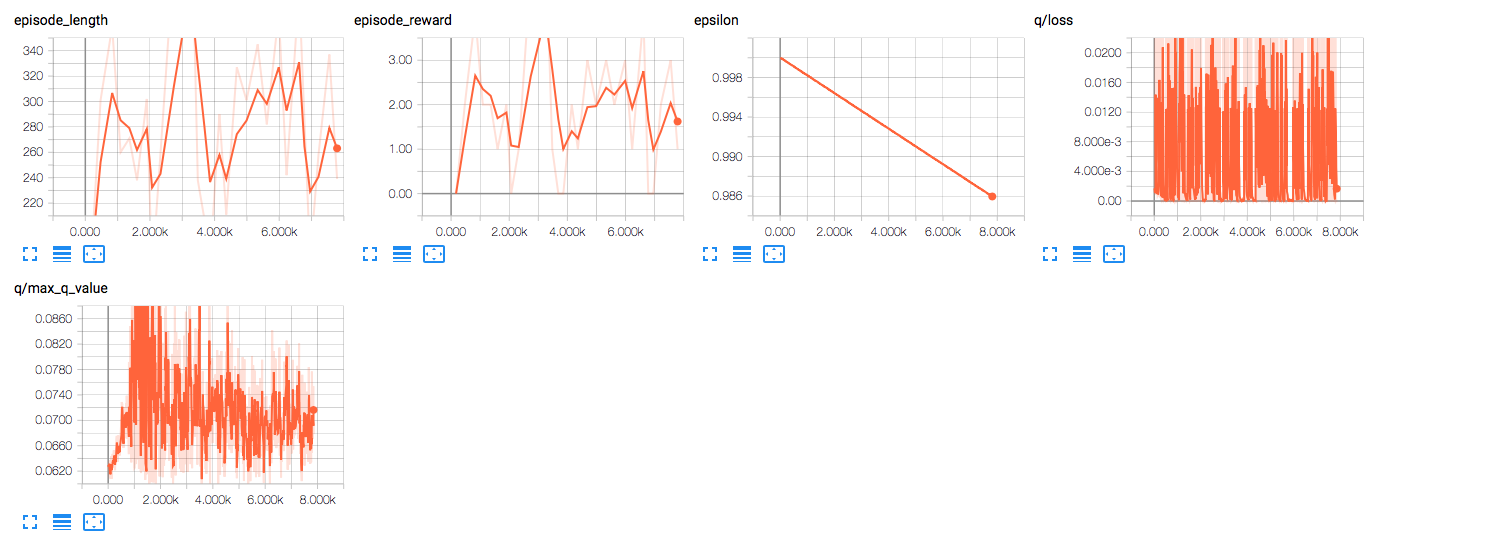
\includegraphics[width=0.8\columnwidth]{figures/tensorboard.png}%
\caption{Initial Experimental Results}%
\label{fig:datastats}%
\end{figure}





\begin{figure}%
\centering
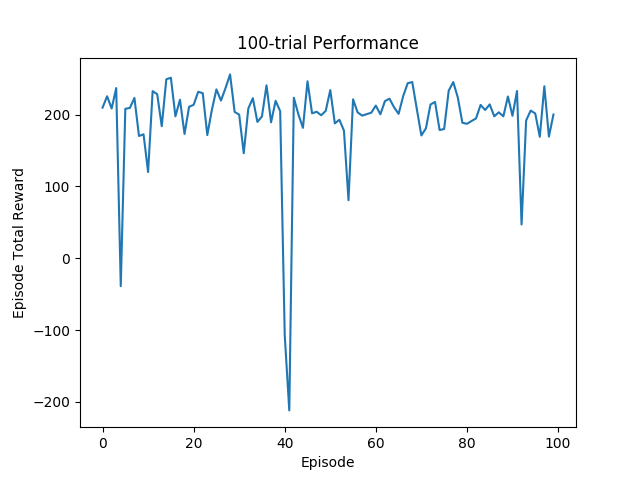
\includegraphics[width=0.6\columnwidth]{figures/evaluate_100.png}%
\caption{Rewards per Episode}%
\label{fig:datastats}%
\end{figure}


